\documentclass[tikz,border=10pt]{standalone}
\usetikzlibrary{calc}
\begin{document}
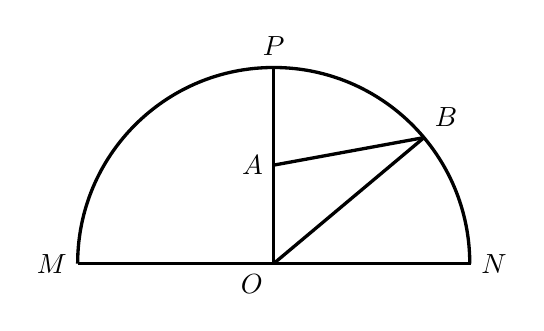
\begin{tikzpicture}[line width=1.2pt, line join=round]
% key points in cm, origin at centre O (TikZ y = (301 - y_px) * 0.0105)
\coordinate (O) at (0,0);
\coordinate (M) at (-2.49,0);
\coordinate (N) at (2.50,0);
\coordinate (P) at (0,2.50);
\coordinate (A) at (0,1.25);
\coordinate (B) at (1.91,1.60);
% upper semicircle from M through P to N (clockwise from 180 deg, so it passes the top)
\draw (M) arc[start angle=180, delta angle=-180, radius=2.49];
% diameter MN
\draw (M) -- (N);
% radius OP (through A), radius OB, chord AB
\draw (O) -- (P);
\draw (O) -- (B);
\draw (A) -- (B);
% point labels
\node[left] at (M) {$M$};
\node[right] at (N) {$N$};
\node[below left] at (O) {$O$};
\node[above] at (P) {$P$};
\node[left] at (A) {$A$};
\node[above right] at (B) {$B$};
\end{tikzpicture}
\end{document}